\section{Chapter 1}
\subsection{Exercises}

\begin{sol}{Exercise 1.1}
We use the Pythagorean Theorem, which states that
\[
a^2 + b^2 = c^2
\]
for a right triangle with legs of length $a$ and $b$ and hypotenuse length $c$. Since we know the leg lengths, and want to find the length of the hypotenuse, we apply the Pythagorean Theorem.
\[
6^2 + 8^2 = c^2
\]
\[
36 + 64 = c^2
\]
\[
100 = c^2
\]
\[
c = \pm 10
\]
Since it does not make sense for a side length to be negative, we simply take only the positive square root.
\[
c = 10
\]
\end{sol}

\begin{sol}{Exercise 1.2}
What have you come up with? The answer is within the subsequent text. 
\end{sol}


\begin{sol}{Exercise 1.3}
The answer is within the subsequent text. However, you may have questions that are not answered by the text! Try to do some work on those and see what you can find by playing around. 
\end{sol}


\begin{sol}{Exercise 1.4}
Test some more patterns! For example, here are the next 5. 
\[
1 + 3 + 5 + 7 + 9 + 11 = 36 = 6^2
\]
\[
1 + 3 + 5 + 7 + 9 + 11 + 13 = 49 = 7^2
\]
\[
1 + 3 + 5 + 7 + 9 + 11 + 13 + 15 = 64 = 8^2
\]
\[
1 + 3 + 5 + 7 + 9 + 11 + 13 + 15 + 17 = 81 = 9^2
\]
\[
1 + 3 + 5 + 7 + 9 + 11 + 13 + 15 + 17 + 19 = 100 = 10^2
\]
\end{sol}

\subsection{Problems}
\begin{sol}{Problem 1.1}
This proves the Pythagorean Theorem for all right triangles because we can choose any right triangle with any leg lengths $a$ and $b$, which determine the triangle. Since the identity holds for any side lengths, it proves Pythagorean Theorem for all triangles.
\end{sol}

\begin{sol}{Problem 1.2}
Here are some symbols I used and their definitions (other than addition and common notations used in arithmetic)
\begin{itemize}
\item $\qed$ : Stands for "quod erat demonstradum", which is Latin for "which was to be demonstrated". In this case, it is used to signify the end of the proof.
\item $\implies$ : This arrow means "implies". It shows that one statement being true implies another statement being true.
\item $\therefore$ : Means "therefore"
\end{itemize}
\end{sol}

\begin{sol}{Problem 1.3}
At this stage, you are not expected to write a proof at all! So, I will just demonstrate the logic we used. We counted the area of the larger square in two ways: first, with the outer side length. Second, by counting the areas of each of the triangles and summing them along with the area of the smaller square. Then, since both count the areas for the square, we set them equal, which simplifies to the Pythagorean Theorem.

More formally,
\begin{proof}
Consider the below figure with labelled side lengths. 
\begin{center}
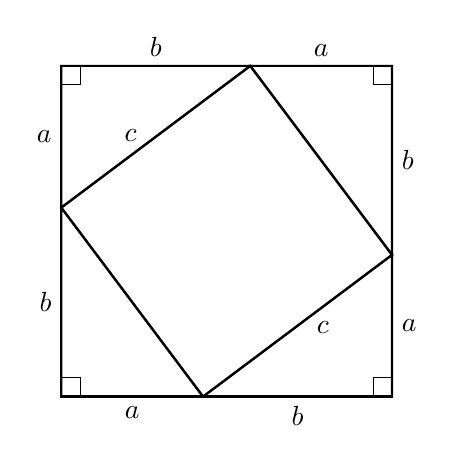
\begin{tikzpicture}[scale=0.6]
  % Outer square
  \draw[thick] (0,0) rectangle (7,7);
  % Inner tilted square
  \draw[thick] (3,0) -- (7,3) -- (4,7) -- (0,4) -- cycle;
  % Triangle outlines
  \draw[thick] (0,0) -- (3,0) -- (0,4) -- cycle;
  \draw[thick] (3,0) -- (7,0) -- (7,3) -- cycle;
  \draw[thick] (7,3) -- (7,7) -- (4,7) -- cycle;
  \draw[thick] (0,4) -- (0,7) -- (4,7) -- cycle;
  % Right angle boxes at OUTER corners
  \draw (0.4,0) -- (0.4,0.4) -- (0,0.4);
  \draw (6.6,0) -- (6.6,0.4) -- (7,0.4);
  \draw (7,6.6) -- (6.6,6.6) -- (6.6,7);
  \draw (0.4,7) -- (0.4,6.6) -- (0,6.6);
  % Outer square side labels
  \node[below] at (1.5,0) {$a$};
  \node[below] at (5.0,0) {$b$};
  \node[right] at (7,1.5) {$a$};
  \node[right] at (7,5.0) {$b$};
  \node[above] at (5.5,7) {$a$};
  \node[above] at (2.0,7) {$b$};
  \node[left]  at (0,5.5) {$a$};
  \node[left]  at (0,2.0) {$b$};
  % Hypotenuse labels
  \node[below right] at (5.2,1.8) {$c$};
  \node[above left]  at (1.8,5.2) {$c$};
\end{tikzpicture}
\end{center}

First, the area of the square on the outside by simply using the outer side length is 
\[
(a+b)^2 = a^2 + 2ab + b^2
\]
Then, the area of each inner triangle is 
\[
\frac{1}{2}ab
\]
The area of the inner square is $c^2$. Since the area of the largest square is the sum of the area of the smaller square and each of the 4 triangles, we have 
\[
a^2 + 2ab + b^2 = c^2 + 4 \cdot \frac{1}{2}ab
\]
which we then simplify
\[
a^2 + 2ab + b^2 = c^2 + 2ab
\]
\[
a^2 + b^2 = c^2
\]
\end{proof}
\end{sol}

\begin{sol}{Problem 1.4}
\begin{proof}
Since we are considering again a proof without words (though I will be explaining it), we represent the summation 
\[
\sum_{i=1}^{n} i
\]
geometrically, with a sort of stair-case-like triangle, shown below. Specifically, in the example shown, $n=5$.
% Diagram 1: single staircase triangle
\begin{center}
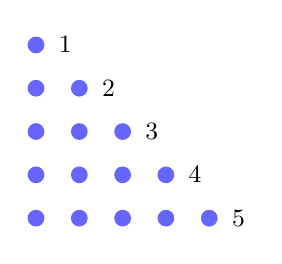
\begin{tikzpicture}[scale=0.55]

  \def\dotradius{0.18}
  \def\n{5}

  % Draw staircase triangle — row k has k dots
  \foreach \row in {1,...,\n}{
    \foreach \col in {1,...,\row}{
      \filldraw[blue!60] (\col, \n+1-\row) circle (\dotradius);
    }
  }

  % Row labels on the right
  \foreach \row in {1,...,\n}{
    \node[right, font=\small] at (\row+0.3, \n+1-\row) {$\row$};
  }

\end{tikzpicture}
\end{center}

The summation is equal to the number of blue dots. We are interested in finding this quantity. To do so, we first add in the same number of extra dots to form a full rectangle, in which there are an equal number of red and blue dots.

% Diagram 2: two triangles forming an n x (n+1) rectangle
\begin{center}
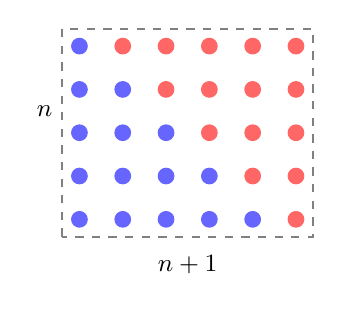
\begin{tikzpicture}[scale=0.55]

  \def\dotradius{0.18}
  \def\n{5}

  % First triangle — blue, staircase going down-left
  \foreach \row in {1,...,\n}{
    \foreach \col in {1,...,\row}{
      \filldraw[blue!60] (\col, \n+1-\row) circle (\dotradius);
    }
  }

  % Second triangle — red, flipped, filling the rest of the rectangle
  \foreach \row in {1,...,\n}{
    \foreach \col in {\row,...,\n}{
      \filldraw[red!60] (\col+1, \n+1-\row) circle (\dotradius);
    }
  }

  % Rectangle outline
  \draw[thick, gray, dashed] (0.6, 0.6) rectangle (\n+1.4, \n+0.4);

  % Dimension labels
  \node[below, font=\small] at ({(\n+2)/2}, 0.4) {$n+1$};
  \node[left,  font=\small] at (0.6, {(\n+2)/2}) {$n$};

\end{tikzpicture}
\end{center}
Then, the number of dots of the blue triangle within this rectangle is exactly $1/2$ the area of the full rectangle (since there are an equal number of blue and red dots within the rectangle). The number of dots within the full rectangle is exactly
\[
n (n+1)
\]
since we have a $n$ by $n+1$ array. Then, we take half to get the formula
\[
\sum_{i=1}^{n}i = \frac{n(n+1)}{2}
\] 
\end{proof}

On a side-note, you may note that the numbers $1, 3, 6, 10, 15, \ldots$ are known as triangular numbers (you can see why from the figure - the dots form a triangle). 
\end{sol}

\begin{sol}{Problem 1.5}
We notice that the sum of the first $n$ cubes is a perfect square. Specifically, the sum of the first $n$ cubes is equal to the square of the sum of the first $n$ positive integers. A natural few questions would be "why?" and "does this always hold?". You may again have more questions and I implore you to explore them! 

We will test the question of "does this always hold?" (a conjecture is a hypothesis, so in this example "this pattern always holds").
\[
1 + 8 + 27 + 64 + 125 = 1^3 + 2^3 + 3^3 + 4^3 + 5^3 = 15^2 = 225
\]
\[
1 + 8 + 27 + 64 + 125 + 216 
\]
\[
= 1^3 + 2^3 + 3^3 + 4^3 + 5^3 + 6^3 = 21^2 = 441
\]
\[
1 + 8 + 27 + 64 + 125 + 216 + 343 
\]
\[
= 1^3 + 2^3 + 3^3 + \cdots + 6^3 + 7^3 = 28^2 = 784
\]
\[
1 + 8 + 27 + 64 + 125 + 216 + 343 + 512 
\]
\[
= 1^3 + 2^3 + \cdots + 8^3 = 36^2 = 1296
\]
Seems like it does!

In summation notation, generalized, the relation is
\[
\sum_{i=1}^{n}i^3 = \left( \sum_{i=1}^{n}i\right)^2
\]
and since we know from the last problem that 
\[
\sum_{i=1}^{n}i = \frac{n(n+1)}{2}
\]
this is
\[
\sum_{i=1}^{n}i^3 = \left( \frac{n(n+1)}{2} \right)^2
\]
\[
= \frac{n^2(n+1)^2}{4} =  \frac{n^4 + 2n^3 + n^2}{4}
\]
which is an interesting identity. The most straightforwards proof of this requires techniques (induction) that we will cover in chapter 2. Other proofs are quite complex, and require some prerequisites in combinatorics.
\end{sol}